\section{Positive and Negative Transfer}\label{sec:cross-domain-transfer}

The same token-normalized formulation produces positive transfer on PTB and WikiText-2 and negative transfer on TinyStories (Table~\ref{tab:cross_domain_transfer}; Figure~\ref{fig:cross_domain_gain}). Every domain has identical gain direction across its three independent student preparations. On TinyStories, CE improves over $S_0$ in all three seeds, so harmful KD is relative to a useful continuation, not simply two unnecessary training arms.

These outcomes establish reproducibility for the tested configurations, not a causal corpus effect. Teachers, data amounts, and student preparation differ across domains. Accepted endpoints are finite; clipping and occasional AMP skips still limit optimization-based interpretation (Appendix~\ref{app:protocols}). Full endpoint NLLs and per-seed gains appear in Appendix~\ref{app:per-seed}.

\begin{table}[t]
\centering
\begin{tabular}{lrr}
\toprule
Dataset & Gain (mean $\pm$ SD) & Signs\\
\midrule
PTB & $+0.144937\pm0.003938$ & 3/3 $+$\\
WikiText-2 & $+0.155665\pm0.007692$ & 3/3 $+$\\
TinyStories & $-0.107219\pm0.000415$ & 3/3 $-$\\
\bottomrule
\end{tabular}
\caption{Paired test-NLL gains from three independent students per corpus; sample SD, $\lambda=5$, $\tau=2$. Both arms select by validation NLL.}
\label{tab:cross_domain_transfer}
\end{table}

\begin{figure*}[!t]
\centering
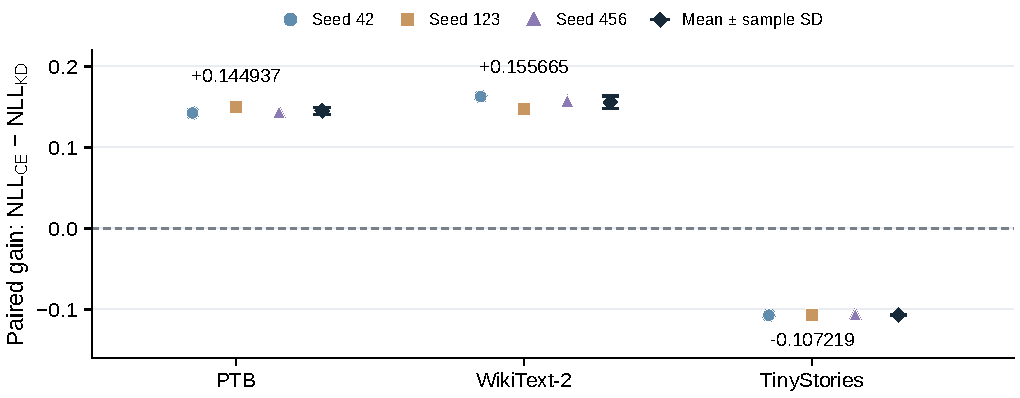
\includegraphics[width=\textwidth]{figures/fig2_cross_domain_gain.pdf}
\caption{CE-relative test-NLL transfer. Dots show independent student seeds; black markers and bars show the mean and sample SD. Positive values favor KD. Teachers and splits are fixed within each corpus.}
\label{fig:cross_domain_gain}
\end{figure*}
